
\documentclass[a4paper,14pt]{extarticle}
\usepackage{cmap}
\usepackage[T2A]{fontenc}
\usepackage[utf8]{inputenc}
\usepackage{setspace}
\usepackage{titlesec}
\usepackage{diagbox}
%\renewcommand{\baselinestretch}{1.5}
\onehalfspacing
\usepackage[english,russian]{babel}
\usepackage{comment}
\usepackage{amsmath,amsfonts,amssymb,mathtext,cite,enumerate,float,indentfirst,floatflt}

\usepackage[left=3cm,right=1cm,
    top=2cm,bottom=2cm,bindingoffset=0cm]{geometry}
		
\renewcommand{\refname}{whatever}	
		
\usepackage{multicol,subcaption,multirow}
\usepackage{graphicx,caption,tocvsec2}

\addto\captionsrussian{\def\refname{СПИСОК ИСПОЛЬЗОВАННЫХ ИСТОЧНИКОВ}}

\usepackage{fancyhdr,fancybox}
\graphicspath{{images_errors_CS/}{images_additional/}{images_errors_EL/}}
\pagestyle{plain}
\fancyhead[L]{\thepage}
\renewcommand{\headrulewidth}{0pt}

\captionsetup[subfigure]{labelformat=simple, labelsep=colon}
\renewcommand{\thesubfigure}{\alph{subfigure}}

\titleformat*{\section}{\large\bfseries}
\titleformat*{\subsection}{\normalsize\bfseries}

\makeatletter
\renewcommand*{\@alph}[1]{%
  \ifcase#1\or а\or б\or в\or г\or
    д\or е\or ё\or ж\or з\or и\or й\or
    к\or л\or м\or н\or о\or п\or р\or с\or\v т\or
    у\or ф\or х\or ц\or ч\or ш\or щ\or ъ\or ы\or ь\or э\or ю\or \v я\else\@ctrerr\fi
}
\makeatother

\begin{document}

\section{Постановка дифференциальной задачи уравнения равновесия}

Для решения общей задачи по определению напряжений и деформаций в деформируемом теле необходимо использовать следующие уравнения равновесия:
\begin{equation}\label{eqGeneral}
\frac{\partial \sigma_{ji}}{\partial x_{j}}=0
\end{equation}
с силовыми граничными условиями
\begin{align}
r &=r_1 \qquad  \sigma_{j i} n_j = -\sigma_{rr}=p_1 \\
r &=r_2 \qquad  \sigma_{j i} n_j = \sigma_{rr}=p_2
\end{align}

После дискретизации задачи с помощью МКЭ, перейдём от задачи (\ref{eqGeneral}) к системе линейных уравнений
\begin{equation}\label{matSLAU}
\textbf{Ku}=\textbf{f}, \qquad u\in \Omega 
\end{equation}
где $\textbf{K}$ - матрица жёсткости, $\textbf{u}$ - вектор перемещений, $\textbf{f}$ - вектор правой части, $\Omega=[r_1, r_2]$.

\subsection{Метод декомпозиции области в дифференциальной постановке}

Разбиваем область $\Omega$ на N пересекающихся подобластей: $\Omega=\bigcup_{i=1}^{N} \Omega_{i}$. 

Решаем задачу \ref{matSLAU} в $\Omega_i$. Обозначим начальное линейное приближение как $u^0$. 

Считаем, что $u^{n}$ известно. Переход $u^n \rightarrow u^{n+1}$ можно записать засчёт следующего итерационного процесса:

\begin{align*}
\frac{\partial \sigma_{ji}}{\partial x_{j}}=0 \qquad  &x\in\Omega_1 \\
\sigma_{rr}=p_{1} \qquad &x\in \partial \Omega_1 \cap \partial \Omega \\
u^{n+\frac{1}{N}}=u^n \qquad &x\in \partial \Omega_1 \cap \Omega_2 
\end{align*}
\begin{align*}
\frac{\partial \sigma_{ji}}{\partial x_{j}}=0 \qquad  &x\in\Omega_k \quad k=2,\ldots,N-1 \\
u^{n+\frac{k}{N}}=u^{n+\frac{k-1}{N}} \qquad &x\in \partial \Omega_k \cap \Omega_{k-1} \\
u^{n+\frac{1}{N}}=u^n \qquad &x\in \partial \Omega_k \cap \Omega_{k+1} 
\end{align*}
\begin{align*}
\frac{\partial \sigma_{ji}}{\partial x_{j}}=0 \qquad  &x\in\Omega_N \\
u^{n+\frac{k}{N}}=u^{n+\frac{k-1}{N}} \qquad &x\in \partial \Omega_N \cap \Omega_{N-1} \\
\sigma_{rr}=p_{N} \qquad &x\in \partial \Omega_N \cap \partial \Omega 
\end{align*}

Для внешних подобластей $\Omega_1$ и $\Omega_N$ решается задача, для которой с одной стороны стоит условие Неймана, с другой стороны - условие Дирихле. Для всех внутренних подобластей $\Omega_2 - \Omega_{N-1}$ с двух сторон стоят условия Дирихле. 

От исходной дифференциальной постановки (\ref{eqGeneral}) можно перейти к слабой постановке задачи и, применяя метод Бубнова - Галёркина, получаем, что на каждой i-ой итерации в $\Omega_j$ нужно решить следующую систему линенйных уравнений:
\begin{equation}
\textbf{$K_{\Omega_j} u_j^i$}=\textbf{$f_j^i$} \qquad j=1,\ldots,N
\end{equation}

\newpage
\section{Результаты решения задачи для упругой трубы. Одномерный случай.}

Рассмотрим случай, когда внутреннее давление $p_a=20$ МПа, внешнее давление $p_b=0$ МПа. Тогда аналитическое радиальное перемещение считается по формуле :
\begin{equation}\label{perem}
u=\frac{\left(1-2\nu\right)\left(1+\nu\right)}{E} \frac{p_a a^2}{b^2-a^2}r+\frac{1+\nu}{E}\frac{a^2 b^2}{r}\frac{p_a}{b^2-a^2}.
\end{equation}

Вычисление аналитического радиального напряжения производится по формуле :
\begin{equation}
\sigma_{rr}=\frac{p_a a^2}{b^2-a^2}-\frac{a^2 b^2}{r^2}\frac{p_a}{b^2 -a^2}
\end{equation}

Вычисление аналитического окружного напряжения производится по формуле :
\begin{equation}
\sigma_{\varphi\varphi}=\frac{p_a a^2}{b^2-a^2}+\frac{a^2 b^2}{r^2}\frac{p_a}{b^2 -a^2}
\end{equation}	

Для решения поставленной задачи примем, что материал цилиндра имеет следующие параметры: модуль Юнга $E - 70000 \:\text{МПА}$ и коэффициент Пуассона $\nu=0.34$. Внутренний радиус цилиндра $a - 10 \:\text{мм}$, внешний радиус цилиндра $b - 20 \:\text{мм}$.

Расчёт относительной погрешности произведён по формуле для нормы, являющейся конечномерным аналогам следующих пространства $L_2$:
\begin{equation}\label{Error_Ot_L2}
\sqrt{\sum_{i=1}^{n} \dfrac{ (u_i^{an}-u_i^{me})^2}{ (u_i^{an})^2 }\dfrac{s_{i}}{\sum{s_i}}}
\end{equation}
где $u^{an}$ - аналитическое решение, $u^{me}$ - численное решение, $s_i$ - полусумма двух шагов $\dfrac{h_i+h_{i+1}}{2}$, $\sum{s_i}$ - сумма всех шагов на всём отрезке. 

Коэффициент относительного захлёста (Overlapping coefficient) - 0.40. Критерии останова - $10^{-5}, 10^{-6}$.

\begin{tabular}{|l|c|c|c|c|}\hline
\diagbox[width=10em]{Кол-во\\подобластей}{Критерий\\ останова $\varepsilon$}&
  $10^{-3}$ & $10^{-4}$ & $10^{-5}$ & $10^{-6}$ \\ \hline
2 & 59 & 92 & 124 & 157 \\ \hline
4 & 205 & 387 & 576 & 765 \\ \hline
10 & 609 & 1691 & 3062 & 4473 \\ \hline
\end{tabular}

Проведена серия расчётов на сетке N=100. Результаты расчётов представлены ниже. 

\begin{figure}[h]
\begin{center}
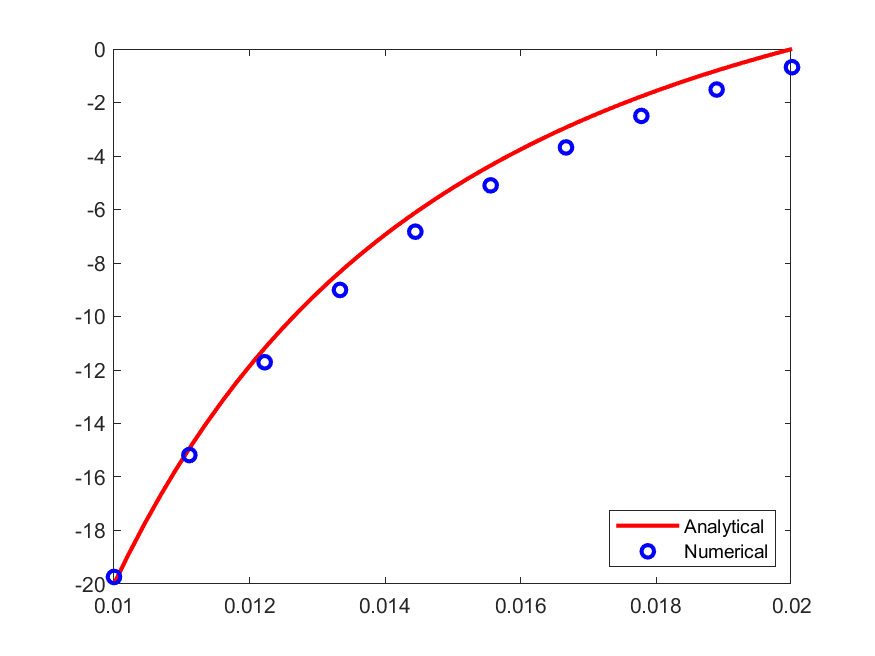
\includegraphics[width=95mm]{graphs/SigmaR.png}
\caption{Зависимость радиальных напряжений от радиуса}
\label{1r}
\end{center}
\end{figure}


\begin{figure}[h]
\begin{center}
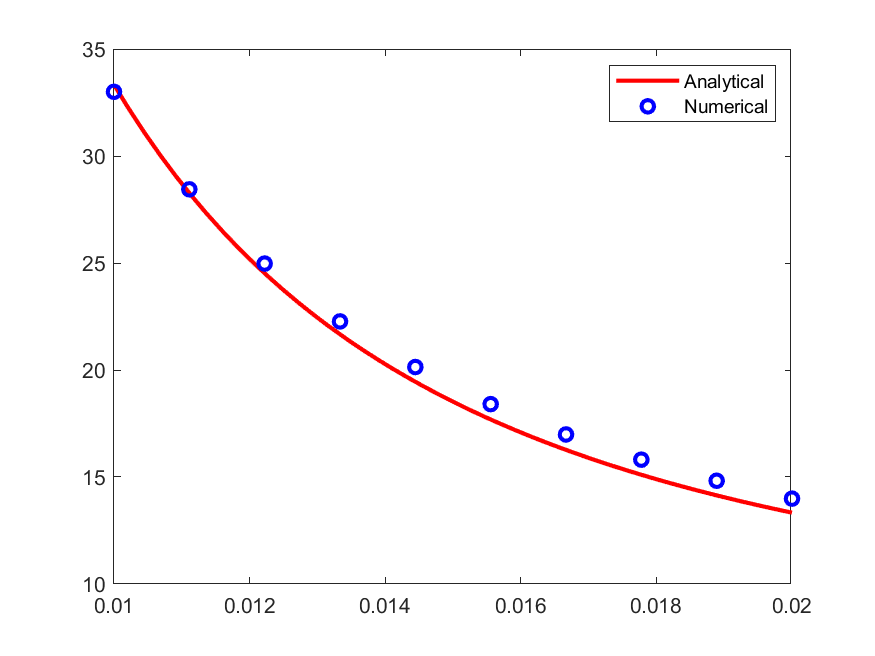
\includegraphics[width=95mm]{graphs/SigmaT.png}
\caption{Зависимость окружных напряжений от радиуса}
\label{1t}
\end{center}
\end{figure}

\begin{table}
\caption{Относительная радиальная погрешность , пространство $L_2$, \\ критерий останова - 1e-5}
\begin{tabular}{|l|c|c|c|}\hline
\diagbox[width=10em]{Кол-во\\подобластей}{Сетка}&
  50 & 100 & 200 \\ \hline
1  & 2.72$\times 10^{-2}$ & 1.36$\times 10^{-2}$ & 6.82$\times 10^{-3}$ \\ \hline	
2  & 2.72$\times 10^{-2}$ & 1.36$\times 10^{-2}$ & 6.81$\times 10^{-3}$ \\ \hline
4  & 2.71$\times 10^{-2}$ & 1.35$\times 10^{-2}$ & 6.76$\times 10^{-3}$ \\ \hline
10 & 2.66$\times 10^{-2}$ & 1.31$\times 10^{-2}$ & 6.19$\times 10^{-3}$ \\ \hline
\end{tabular}
\end{table}

\begin{table}
\caption{Относительная окружная погрешность, пространство $L_2$, \\ критерий останова - 1e-5}
\begin{tabular}{|l|c|c|c|}\hline
\diagbox[width=10em]{Кол-во\\подобластей}{Сетка}&
  50 & 100 & 200 \\ \hline
1  & 1.14$\times 10^{-2}$ & 5.69$\times 10^{-3}$ & 2.83$\times 10^{-3}$ \\ \hline	
2  & 1.15$\times 10^{-2}$ & 5.78$\times 10^{-3}$ & 2.93$\times 10^{-3}$ \\ \hline
4  & 1.25$\times 10^{-2}$ & 6.34$\times 10^{-3}$ & 3.49$\times 10^{-3}$ \\ \hline
10 & 1.63$\times 10^{-2}$ & 1.06$\times 10^{-2}$ & 7.89$\times 10^{-3}$ \\ \hline
\end{tabular}
\end{table}

\begin{table}
\caption{Относительная радиальная погрешность, пространство $L_2$, \\ критерий останова - 1e-6}
\begin{tabular}{|l|c|c|c|}\hline
\diagbox[width=10em]{Кол-во\\подобластей}{Сетка}&
  50 & 100 & 200 \\ \hline
1  & 2.72$\times 10^{-2}$ & 1.36$\times 10^{-2}$ & 6.82$\times 10^{-3}$ \\ \hline	
2  & 2.72$\times 10^{-2}$ & 1.36$\times 10^{-2}$ & 6.82$\times 10^{-3}$ \\ \hline
4  & 2.72$\times 10^{-2}$ & 1.36$\times 10^{-2}$ & 6.81$\times 10^{-3}$ \\ \hline
10 & 1.72$\times 10^{-2}$ & 1.35$\times 10^{-2}$ & 6.81$\times 10^{-3}$ \\ \hline
\end{tabular}
\end{table}

\begin{table}
\caption{Относительная окружная погрешность, пространство $L_2$, \\ критерий останова - 1e-6}
\begin{tabular}{|l|c|c|c|}\hline
\diagbox[width=10em]{Кол-во\\подобластей}{Сетка}&
  50 & 100 & 200 \\ \hline
1  & 1.14$\times 10^{-2}$ & 5.69$\times 10^{-3}$ & 2.83$\times 10^{-3}$ \\ \hline	
2  & 1.14$\times 10^{-2}$ & 5.71$\times 10^{-3}$ & 2.84$\times 10^{-3}$ \\ \hline
4  & 1.15$\times 10^{-2}$ & 5.75$\times 10^{-3}$ & 2.91$\times 10^{-3}$ \\ \hline
10 & 1.19$\times 10^{-2}$ & 6.18$\times 10^{-3}$ & 3.08$\times 10^{-3}$ \\ \hline
\end{tabular}
\end{table}

\end{document}

